\chapter{Stato dell'Arte}
Questa Tesi si colloca nell'ambito del posizionamento ferrotramviario.\\*
Il problema del posizionamento esiste tanto nel contesto ferroviario quanto nel contesto ferrotramviario, dal momento che il secondo nasce come derivazione dal primo. In questo capitolo vengono introdotte le principali caratteristiche dei sistemi ferrotramviari e si descrive lo stato dell'arte nell'ambito del posizionamento ferrotramviario, al fine di introdurre gli argomenti trattati nel seguito.
\section{Sistemi Ferroviari e Ferrotramviari}
\`E possibile schematizzare un Sistema Ferroviario, o Ferrotramviario, come un insieme di vetture vincolate a muoversi lungo una traccia fissa.\\*
Questa schematizzazione vale per qualsiasi sistema di trasporto ferroviario o ferrotramviario a prescindere dalla sua scala in termini di veicoli transitanti ed estensione geografica. Ci\'o che invece differenzia un Sistema Ferroviario da un Sistema Ferrotramviario sono:
\begin{itemize}
		\item Le caratteristiche fisiche del treno, come lunghezza e massa;
		\item Le caratteristiche geografiche dell'ambiente operativo;
		\item Gli scopi del trasporto.
\end{itemize}
In generale, nel trasporto ferroviario si utilizzano treni caratterizzati da grandi dimensioni, che trasportano persone o merci su lunghe percorrenze, e che operano pertanto prevalentemente in ambienti extra urbani. \\*
Nel trasporto ferrotramviario, di contro, si utilizzano vetture dalle ridotte dimensioni, pi\'u leggere di quelle usate nei sistemi ferroviari, e che hanno lo scopo di rappresentare un'alternativa per il cittadino all'utilizzo di mezzi privati durante i suoi spostamenti all'interno di un'area metropolitana. Quest'ultima caratteristica implica che l'ambiente operativo di un sistema ferrotramviario sia radicalmente diverso da quello di un sistema ferroviario: i treni si muovono lungo rotaie installate su strade urbane, quindi il traffico ferrotramviario \`e fuso con il traffico cittadino, come mostrato in figura \ref{fig:tramschema}.\\*
\begin{figure}[h]
		\centering
		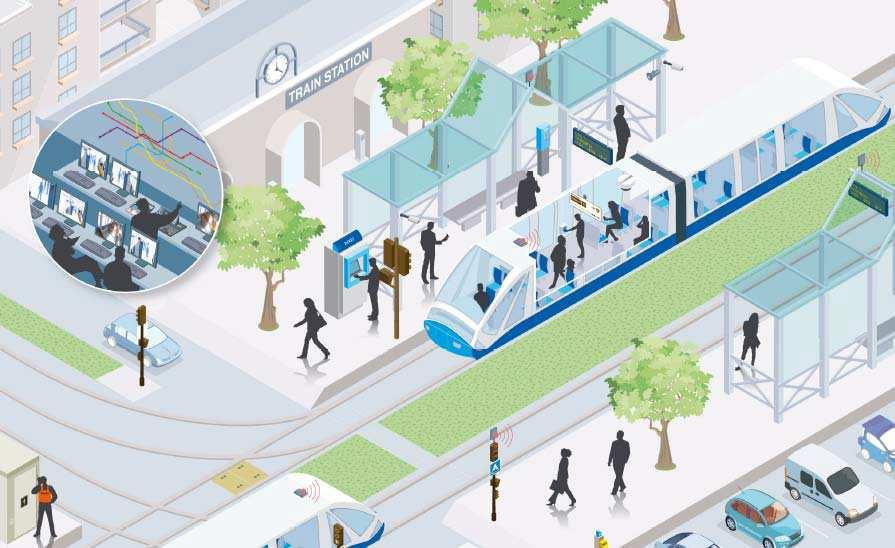
\includegraphics[width=0.7\linewidth]{img/twschema}
		\caption{Schema di un tipico scenario tramviario}
		\label{fig:tramschema}
\end{figure}
\section{Il problema del posizionamento}
Per posizionamento ferroviario, si intende la valutazione della posizione di un treno all'interno di una traccia ferroviaria. Esso esiste tanto nel contesto ferrotramviario quanto nel contesto ferroviario classico.\\*
Tale posizione viene espressa come progressiva chilometrica rispetto all'origine della linea oppure.\\*
Il problema del posizionamento sorge nel momento in cui, per ragioni di rotta, un treno ha necessit\`a di spostarsi da una sezione di binario, anche detta traccia, ad un'altra. Questa operazione di scambio \`e offerta dal sistema di \emph{interlocking} \cite{interlocking}. Tale sistema \`e detto \emph{safety-critical} \cite{safetycritical}, pertanto offre una funzionalit\`a che deve rispettare adeguati standard di sicurezza.\\*
Gli odierni sistemi di posizionamento si basano principalmente sull'utilizzo di strumenti installati a terra, che hanno lo scopo di rilevare il passaggio di un treno, e quindi di interagire con il sistema di \emph{interlocking} della traccia al fine di garantire, con un elevato livello di confidenza, un transito sicuro dei mezzi.
\subsubsection{Odierne Tecniche di Posizionamento}
I sistemi di posizionamento attualmente in uso hanno come nucleo essenziale il sistema di \emph{interlocking}, il quale si fa carico di offrire al treno un attraversamento sicuro di una \emph{Junction Area (JA)}. Una JA \`e un punto della linea ferroviara in cui il treno pu\'o cambiare direzione, e occupare una nuova traccia di binario.\\*
La nuova traccia da occupare potrebbe avere particolari vincoli sul numero di treni contemporaneamente transitanti, ed in ogni caso lo scambio di rotaia deve essere corretto ed avvenire in sicurezza, in quanto occupare la traccia sbagliata potrebbe avere ripercussioni finanche catastrofiche. \cite{marocchini}\\*
Un sistema di \emph{interlocking} \`e composto dai seguenti elementi:
-\begin{itemize}
		\item \emph{Switch Control Unit (UCS)}:\\*
		Piattaforma certificata \texttt{SIL-3} \cite{sil} che rappresenta il nucleo del sistema di \emph{interlocking} e che implementa l'intera logica di gestione di una JA. Un UCS dispone di un'interfaccia di \emph{Input/Output} verso gli elementi di \emph{interlocking} installati a terra e ne consente un controllo sicuro in accordo allo standard \texttt{SIL-3}.
	\begin{figure}[h]
		\centering
				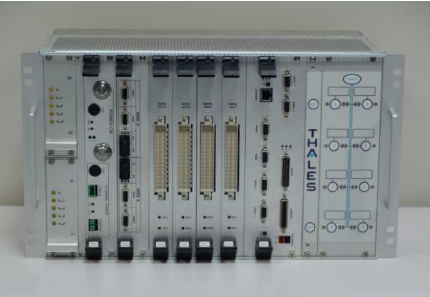
\includegraphics[width=0.7\linewidth]{img/ucs}
				\caption{UCS}
				\label{fig:ucs}
		\end{figure}\clearpage
		\item Conta Assi:\\*
		Il Conta Assi, o in inglese \emph{Axle Counter} (AC), \`e un sistema certificato \texttt{SIL-3} che ha lo scopo di rilevare la presenza del treno e fornire quindi lo stato di occupazione della sezione di traccia in cui l'AC \`e installato.
	\begin{figure}[h]
			\centering
			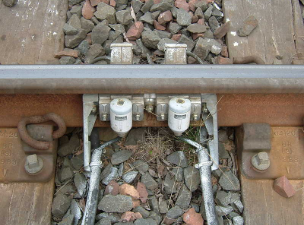
\includegraphics[width=0.7\linewidth,height=7.1cm]{img/axlecounter}
			\caption{Conta Assi}
			\label{fig:ac}
		\end{figure}
		\item \emph{Point Machines}:\\*
		Le \emph{Point Machines} infine, sono degli strumenti certificati \texttt{SIL-3} che hanno lo scopo di direzionare le rotaie verso una determinata sezione di traccia.
		\begin{figure}[h]
				\centering
				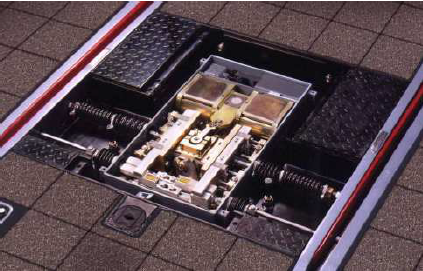
\includegraphics[width=0.7\linewidth]{img/pointmachine}
				\caption{\emph{Point Machine}}
				\label{fig:pointmachine}
			\end{figure}
	\end{itemize}
L'intero sistema di \emph{interlocking} viene attivato dai \emph{Track Circuit}. Questi apparati sono installati a terra prima di ciascuna JA, e segnalano al sistema di \emph{interlocking} l'avvicinamento di un treno alla successiva JA.
\subsection{Criticit\`a}
Le attuali tecniche di posizionamento richiedono un intervento trascurabile di computer installati a bordo e una grande quantit\`a di apparati installati a terra. Mentre i computer di bordo non forniscono in generale funzionalit\`a legate alla \emph{safety}, gli apparati installati a terra sono costosi e hanno un impatto ambientale non trascurabile.\\*
\`E possibile considerare il treno e il computer di bordo come un unico sistema, ossia il treno viene modellato come un \emph{Cyber-Physical System}.\\*
Un \emph{Cyber-Physical System} (CPS) \`e un sistema composto da una parte \emph{fisica} e da una parte \emph{cyber}. Il sottosistema fisico \`e composto da sensori e attuatori che hanno rispettivamente lo scopo di rilevare lo stato dell'ambiente circostante e di alterarlo se necessario. Il sottosistema \emph{cyber} \`e essenzialmente un elaboratore, che dispone di processore, memoria, e interfacce I/O verso i sensori, gli attuatori, ed eventuali operatori  umani. \cite{cps}\cite{cecca} Una tale architettura di sistema, permette di sfruttare le capacit\`a di calcolo dei moderni processori per implementare algoritmi anche molto complessi per il \emph{processing} di grandi quantit\`a di dati provenienti dai sensori.\\*
Lo scopo della Tesi \`e quello di mostrare i risultati sperimentali delle campagne di analisi condotte su di un innovativo sottosistema di posizionamento. Tale sottosistema ha lo scopo di stimare la posizione di un treno attraverso l'uso combinato di un insieme di sensori installati bordo treno, e al fine di integrarne le misure, queste dovranno essere processate da un algoritmo noto come \emph{Sensor Fusion Algorithm} (SFA).\cite{datafuse} \cite{sfarailway} 